\chapter{\babTiga}
\label{bab:3}


\section{Mekanisme \f{Attention}}
Mekanisme \f{Attention} dapat ditinjau sebagai \f{Dictinoary Lookup}, yaitu untuk sebuah vektor kueri $\mathbf{q}$ dan sekumpulan pasangan terurut vektor $\mathcal{KV} = \{(\mathbf{k}_1, \mathbf{v}_2), (\mathbf{k}_2, \mathbf{v}_2), \dots, (\mathbf{k}_n, \mathbf{v}_n)\}$, mekanisme \f{attention} akan mengembalikan vektor nilai $\mathbf{v}_i$ yang memiliki vektor kunci $\mathbf{k}_i$ yang cocok dengan vektor kueri $\mathbf{q}$. \equ~\ref{equ:hard-attention-start} menunjukkan bagaimana mekanisme \f{attention} dilakukan.
\begin{align}
	\label{equ:hard-attention-start}
	\text{Attention}(\mathbf{q}, \mathbf{K}, \mathbf{V}) &= [\alpha_{1}, \alpha_{2}, \dots, \alpha_{n}]\mathbf{V} \in \mathbb{R}^{d_v},
\end{align}
	dengan keterangan sebagai berikut:
	\begin{flalign*}
		\mathbf{K}&= \begin{bmatrix}
			\mathbf{k}_1 \\
			\mathbf{k}_2 \\
			\vdots \\
			\mathbf{k}_n
		\end{bmatrix} \in \mathbb{R}^{n \times d_k},&& \\
		\mathbf{V} &= \begin{bmatrix}
			\mathbf{v}_1 \\
			\mathbf{v}_2 \\
			\vdots \\
			\mathbf{v}_n
		\end{bmatrix} \in \mathbb{R}^{n \times d_v},&& \\
	\alpha_i &= 
	\begin{cases}
		1, & \text{jika } i = \arg\max_{j} f_{attn}(\mathbf{q}, \mathbf{k}_j) \\
	0, & \text{lainnya}
	\end{cases}.
	\end{flalign*}

	$f_{attn}(\mathbf{q}, \mathbf{k})$ adalah fungsi atensi yang menghitung nilai atensi antara vektor kueri $\mathbf{q}$ dan vektor kunci $\mathbf{k}$. $\alpha_i$ pada persamaan di atas disebut sebagai bobot atensi dan nilai $f_{attn}(\mathbf{q}, \mathbf{k})$ disebut sebagai nilai atensi.
	
	Sebagai contoh, untuk $\mathbf{q}= [1,2]$, $\mathcal{KV} = \{([2,1],[1,0]), ([1,2],[0,1])\}$ serta fungsi $f_\text{attn}(\mathbf{q}, \mathbf{k}) =\mathbf{q}\cdot \mathbf{k}$, nilai dari $\text{Attention}( \mathbf{q}, \mathbf{K}, \mathbf{V})$ adalah $[0,1]$, karena nilai maksimal $f_\text{attn}$ terjadi ketika $\mathbf{k} = [1,2]$. 

	Mekansime \f{attention} pada \equ~\ref{equ:hard-attention-start} disebut sebagai \f{hard attention} karena hanya satu vektor nilai $\mathbf{v}_i$ yang dipilih dari sekumpulan vektor nilai $\mathbf{V}$. Berbeda dengan \f{hard attention}, \f{soft attention} mengambil seluruh vektor nilai $\mathbf{V}$ dan menghitung bobot $\alpha_i$ untuk setiap vektor nilai $\mathbf{v}_i$ dengan fungsi \f{softmax}. Hasil dari \f{soft attention} adalah rata-rata terbobot dari seluruh vektor nilai $\mathbf{V}$. \equ~\ref{equ:soft-attention-start} menunjukkan bagaimana mekanisme \f{soft attention} dilakukan.
	\begin{align}
		\label{equ:soft-attention-start}
		\text{Attention}(\mathbf{q}, \mathbf{K}, \mathbf{V}) &= [\alpha_{1}, \alpha_{2}, \dots, \alpha_{n}]\mathbf{V} \in \mathbb{R}^{d_v},
	\end{align}
	dengan nilai $\alpha_i$ yang dihitung seperti persamaan berikut:
	\begin{flalign*}
		\alpha_{i}(\mathbf{q},\mathbf{k}_i) &= \text{Softmax}_i(\bm{\alpha}) = \frac{\exp(f_{attn}(\mathbf{q}, \mathbf{k}_i))}{\sum_{j=1}^{n} \exp(f_{attn}(\mathbf{q}, \mathbf{k}_j))}.
	\end{flalign*}

	\begin{figure}
		\centering
		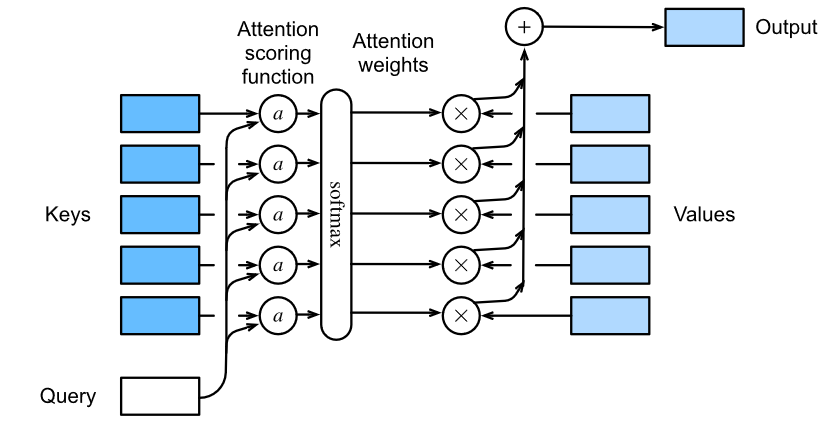
\includegraphics[width=1\textwidth]{assets/pics/softattention.png}
		\captionsource{Ilustrasi dari mekanisme \f{soft attention}.}{ \citep{zhang2023dive}.}
		\label{fig:soft-attention}
	\end{figure}


	Dengan rata-rata terbobot dari $\mathbf{V}$, transformasi \f{soft attention} terturunkan. Hal ini merupakan syarat \f{fundamental} yang harus dimiliki oleh sebuah model \f{deep learning}.

	Sebagai contoh, hasil dari $\text{Attention}(\mathbf{q}, \mathbf{K}, \mathbf{V})$ untuk $\mathbf{q}= [1,2]$, $\mathcal{KV} = \{([2,1],[0,1]), ([1,2],[1,0])\}$ serta fungsi $f_\text{attn}(\mathbf{q}, \mathbf{k}) =\mathbf{q}\cdot \mathbf{k}$ adalah $0.268 [0,1] + 0.732 [1,0] = [0.732, 0.268]$ dengan $\alpha_1 = \frac{\exp(4)}{\exp(4) + \exp(5)} \approx 0.268$ dan $\alpha_2 = \frac{\exp(5)}{\exp(4) + \exp(5)} \approx 0.732$.

	Pada kasus kumpulan kueri $\mathcal{Q} = \{\mathbf{q}_1, \mathbf{q}_2, \dots, \mathbf{q}_m\}$, mekanisme \f{attention} untuk setiap triplet $(\mathbf{q}_i, \mathbf{K}, \mathbf{V})$ dapat dihitung secara bersamaan seperti yang ditunjukkan pada \equ~\ref{equ:soft-attention-matrix-start}.
	\begin{align}
		\label{equ:soft-attention-matrix-start}
		\text{Attention}(\mathbf{Q}, \mathbf{K}, \mathbf{V}) &= \mathbf{A} \mathbf{V} \in \mathbb{R}^{m \times d_v},
	\end{align}
	dengan:
	\begin{flalign*}
		\mathbf{Q} &= \begin{bmatrix}
			\mathbf{q}_1 \\
			\mathbf{q}_2 \\
			\vdots \\
			\mathbf{q}_m
		\end{bmatrix} \in \mathbb{R}^{m \times d_k}, && \\
		\mathbf{A} &= \begin{bmatrix}
			\bm{\alpha}_1 \\
			\bm{\alpha}_2 \\
			\vdots \\
			\bm{\alpha}_m
		\end{bmatrix} = \begin{bmatrix}
			\alpha_{11} & \alpha_{12} & \dots & \alpha_{1n} \\
			\alpha_{21} & \alpha_{22} & \dots & \alpha_{2n} \\
			\vdots & \vdots & \ddots & \vdots \\
			\alpha_{m1} & \alpha_{m2} & \dots & \alpha_{mn} \\
		\end{bmatrix} \in \mathbb{R}^{m \times n}, && \\
		\alpha_{ij}(\mathbf{q}_i, \mathbf{k}_j) &= \text{Softmax}_j(\mathbf{\alpha}_i) = \frac{\exp(f_{attn}(\mathbf{q}_i, \mathbf{k}_j))}{\sum_{k=1}^{n} \exp(f_{attn}(\mathbf{q}_i, \mathbf{k}_k))} \in \mathbb{R}, &&
	\end{flalign*}
	 dan $\alpha_{ij}$ adalah bobot yang menunjukkan bobot atensi antara vektor kueri $\mathbf{q}_i$ dengan vektor kunci $\mathbf{k_j}$. 

	\subsection{\f{Attention} Parametrik}
	Mekanisme \f{attention} yang dilakukan oleh \cite{transformerori} merupakan mekanisme \f{attention} parametrik. Pada mekanisme \f{attention} parametrik, nilai $f_{\text{attn}}$ antar vektor kueri $\mathbf{q}$ dan $\mathbf{v}$ dibandingkan pada ruang vektor yang akan dipelajari (\f{learned embedding space}) daripada ruang vektor aslinya. Sebagai contoh, untuk suatu kueri $\mathbf{q}\in \mathbb{R}^{d_q}$, dan vektor kunci $\mathbf{k} \in \mathbb{R}^{d_k}$, \f{additive attention} yang diperkenalkan oleh \cite{bahdanau2016neural} menghitung nilai keserupaan antara $\mathbf{q}$ dan $\mathbf{k}$ seperti pada \equ~\ref{equ:additive-attention}
	\begin{align}
	\label{equ:additive-attention}
	f_{attn}(\mathbf{q} \mathbf{W}^q, \mathbf{k} \mathbf{W}^k) &= (\mathbf{q} \mathbf{W}^q  + \mathbf{k} \mathbf{W}^k)  \mathbf{W}^{\text{out}} \in \mathbb{R},
	\end{align}
	dengan $\mathbf{W}^q \in \mathbb{R}^{d_q \times d_{\text{attn}}}, \mathbf{W}^k \in \mathbb{R}^{d_k \times d_{\text{attn}}}, \mathbf{W}_{\text{out}} \in \mathbb{R}^{d_{\text{attn}} \times 1}$ adalah matriks parameter yang akan diestimasi selama proses pelatihan. Contoh \f{attention} parametrik yang lebih sederhana adalah \f{dot-product attention}. Fungsi $f_{attn}$ yang digunakan adalah perkalian titik antara $\mathbf{q}$ dan $\mathbf{k}$ di ruang vektor yang dipelajari (\f{learned embedding space}). \equ~\ref{equ:dot-product-attention} menunjukkan bagaimana \f{dot-product attention} dihitung.
	\begin{align}
		\label{equ:dot-product-attention}
		f_{attn}(\mathbf{q} \mathbf{W}^q, \mathbf{k} \mathbf{W}^k) = (\mathbf{q} \mathbf{W}^q) (\mathbf{k} \mathbf{W}^k)^{\top}.
	\end{align}

\section{Transformer}
	\begin{figure}
		\centering
		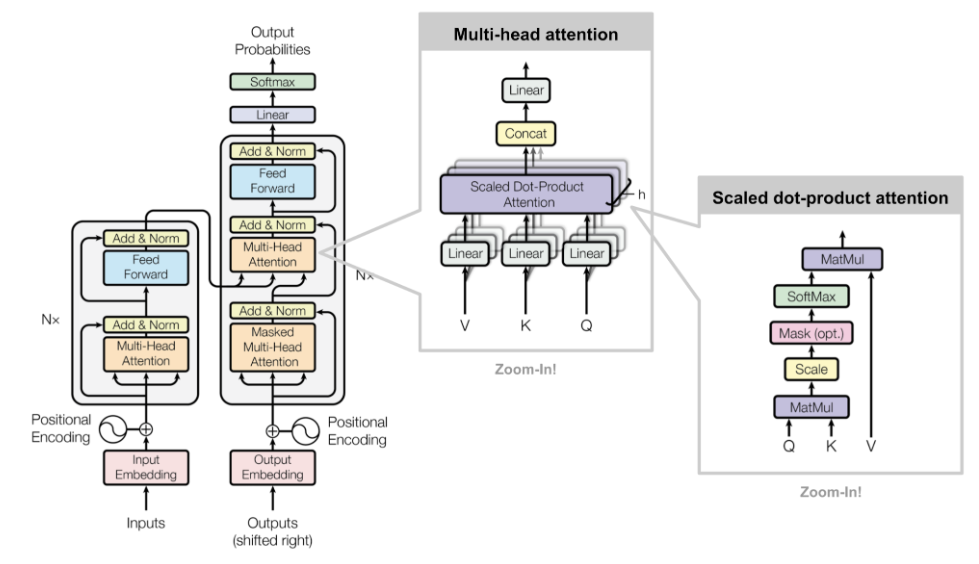
\includegraphics[width=1\textwidth]{assets/pics/lilianweng-transformer.png}
		\caption{Arsitektur \f{transformer} \citep{weng2018attention}.}
		\label{fig:transformer}
	\end{figure}
	\f{Transformer} merupakan Arsitektur \f{deep learning} yang pertama kali diperkenalkan oleh \cite{transformerori}. Awalnya Transformer  merupakan model \f{sequance to sequance} yang diperuntukkan untuk permasalahan mesin translasi neural (\f{neural machine translation}). Namun, sekarang \f{transformer} juga digunakan untuk permasalahan pemrosesan bahasa alami lainnya. model-model yang berarsitektur \f{transformer} menjadi model \f{state-of-the-art} untuk permasalahan pemrosesan bahasa alami lainnya, seperti \f{question answering}, \f{sentiment analysis}, dan \f{named entity recognition}.
 
	Berbeda dengan arsitektur mesin translasi terdahulu, transformer tidak mengunakan \f{recurrent neural network} (RNN) atau \f{convolutional neural network} (CNN), melainkan transformer adalah model \f{feed foward network} yang dapat memproses seluruh \f{input} pada barisan secara paralel. Untuk menggantikan kemampuan RNN dalam mempelajari ketergantungan antar \f{input} yang berurutan dan kemampuan CNN dalam mempelajari fitur lokal, transformer bergantung pada mekanisme \f{attention}.

	Terdapat tiga jenis \f{attention} yang digunakan dalam model \f{transformer} \citep{transformerori}:
	\begin{enumerate}
		\item \f{Encoder self-attention}: menggunakan barisan \f{input} yang berupa barisan token atau kata sebagai masukan untuk menghasilkan barisan representasi kontekstual, berupa vektor, dari \f{input}. Setiap representasi token tersebut memiliki ketergantungan dengan token lainnya dari barisan \f{input}.
		\item \f{Decoder self-attention}: menggunakan barisan \f{target} yang berupa kalimat terjemahan parsial, barisan token, sebagai masukan untuk menghasilkan barisan representasi kontekstual (vektor) dari \f{target}. Setiap representasi token tersebut memiliki ketergantungan dengan token sebelumnya dalam urutan masukan.
		\item \f{Decoder-encoder attention}: menggunakan barisan representasi kontekstual dari \f{input}, dan barisan representasi kontekstual dari \f{target} untuk menghasilkan token berikutnya yang merupakan hasil prediksi dari model. Barisan \f{target} yang digabung dengan token hasil prediksi tersebut akan menjadi barisan \f{target} untuk prediksi selanjutnya.
	\end{enumerate}
	Arsitektur dari \f{transformer} terdiri dari pasangan encoder-decoder. Aristektur dari \f{transformer} dapat dilihat pada \pic~\ref{fig:transformer}. Lapisan \f{encoder} berfungsi untuk memahami konteks suatu kata dalam teks atau kalimat, sementara lapisan \f{decoder} digunakan untuk menyelesaikan masalah translasi menuju bahasa berbeda. Pada permasalahan klasifikasi seperti analisis sentimen dan pemeringkatan teks, lapisan \f{decoder} tidak digunakan. pada permasalahan tersebut, \f{output} dari lapisan \f{encoder} yang digunakan sebagai masukan untuk lapisan \f{classifier}. \sect~\ref{sec:token-embedding} hingga \sect~\ref{sec:encoder} menjelaskan arsitektur model \f{transformer encoder} dan berbagai mekanisme yang menyusun model \f{transformer}.

	\subsection{\f{Token Embedding (Input Embedding)}}
	\label{sec:token-embedding}
	\begin{figure}
		\centering
		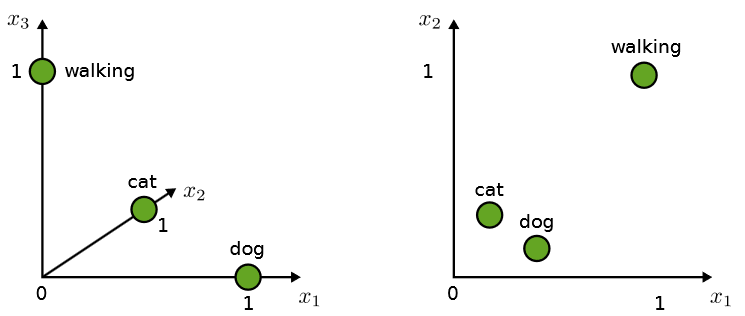
\includegraphics[width=1\textwidth]{assets/pics/token-embedding.png}
		\captionsource{Ilustrasi dari representasi token. Gambar kiri menunjukkan representasi token dengan \f{one-hot encoding}, sedangkan gambar kanan menunjukkan representasi token dengan \f{token embedding}.}{\citep{geiger2022deeplearning}.}
		\label{fig:token-embedding}
	\end{figure}
	Perlu diingat kembali bahwa \f{input} dari \f{Attention} (dan tentunya \f{transformer}) adalah barisan vektor. Jika \f{Attention} ingin dapat digunakan pada permasalahan bahasa, barisan kata atau subkata (selanjutnya disebut token) harus terlebih dahulu diubah menjadi barisan vektor.

	Representasi vektor dari token yang paling sederhana adalah dengan \f{one-hot encoding}. Andaikan $\mathcal{T} = \{t_1, t_2, \dots, t_{|\mathcal{T}|}\}$ adalah semua kemungkinan token yang mungkin muncul dalam permasalahan bahasa yang ingin diselesaikan. Untuk sembarang barisan token $t = (t_{i_1}, t_{i_2}, \dots, t_{i_L})$, representasi vektor dari token $t_{i_j}$ adalah vektor $\mathbf{oh}_{i_j} = [0, \dots, 0, 1, 0, \dots, 0] \in \mathbb{R}^{|\mathcal{T}|}$, dengan nilai 1 pada indeks ke $j$ dan nilai 0 pada indeks lainnya. \f{One-hot encoding} tentunya memiliki kelemahan:
	\begin{enumerate}
		\item Vektor yang dihasilkan adalah \f{sparse vector}, dan ukuran vektor yang dihasilkan cukup besar, yaitu $|\mathcal{T}|$.
		\item Representasi token yang buruk. Operasi vektor yang dilakukan pada \f{one-hot encoding} tidaklah bermakna. Misalnya, Jarak antar token akan selalu sama pada \f{one-hot encoding}, yaitu $\sqrt{2}$.
	\end{enumerate}

	Untuk Mengatasi kekurangan dari representasi \f{one-hot encoding}, representasi yang digunakan adalah vektor padat yang akan dipelajari ketika proses pelatihan. Misalkan $\mathbf{E}_{\mathcal{T}} \in \mathbb{R}^{|\mathcal{T}| \times d_{\text{token}}}$ adalah matriks parameter yang merupakan representasi vektor padat dari seluruh token ada. \equ~\ref{equ:token-embedding-start} hingga \equ~\ref{equ:token-embedding-end} menunjukkan bagaimana representasi vektor dari barisan suatu token $t$ dihitung. 
	\begin{align}
		\label{equ:token-embedding-start}
		\text{Embed}(t) &= \mathbf{E}_{t} = \begin{bmatrix}
			\mathbf{e}_{i_1} \\
			\mathbf{e}_{i_2} \\
			\vdots \\
			\mathbf{e}_{i_L}
		\end{bmatrix} \in \mathbb{R}^{L \times d_{\text{token}}}, \\
		\mathbf{e}_{i_j} &= \mathbf{oh}_{i_j} \mathbf{E}_{\mathcal{T}} \in \mathbb{R}^{d_{\text{token}}}.
		\label{equ:token-embedding-end}
	\end{align}

	\pic~\ref{fig:token-embedding} mengilustrasikan perbedaan antara \f{one-hot encoding} dan \f{token embedding}. Pada representasi token dengan vektor padat, vektor yang secara semantik atau sintaksis mirip akan memiliki jarak yang lebih dekat. Selain itu, biasanya representasi token dengan vektor padat memiliki dimensi $d_{\text{token}}$ yang lebih kecil daripada \f{one-hot encoding} yang memiliki dimensi $|\mathcal{T}|$.

	\subsection{\f{Scaled Dot-Product Attention}}
	\label{sec:scaled-dot-product-attention}

	\f{Scaled dot-product attention} adalah mekanisme \f{Attention} parametrik yang digunakan dalam \f{transformers}. \f{Scaled dot-product attention} menghitung keserupaan antara vektor kueri $\mathbf{q}$ dan vektor kunci $\mathbf{k}$ pada ruang vektor yang dipelajari (\f{learned embedding space}) dengan fungsi keserupaan $f_{attn}(\mathbf{q} \mathbf{W}^q, \mathbf{k}\mathbf{W}^k) $ adalah perkalian titik antara $\mathbf{qW}^q$ dan $\mathbf{kW}^k$ yang kemudian dibagi dengan $\sqrt{d_{attn}}$, seperti yang ditunjukkan \equ~\ref{equ:scaled-dot-product-attention}.
	\begin{align}
		\label{equ:scaled-dot-product-attention}
		f_{attn}(\mathbf{q} \mathbf{W}^q, \mathbf{k} \mathbf{W}^k) &= \frac{\mathbf{q} \mathbf{W}^q (\mathbf{k} \mathbf{W}^k)^{\top}}{\sqrt{d_{attn}}} \in \mathbb{R}.
	\end{align}
	dengan $\mathbf{W}^q \in \mathbb{R}^{d_q \times d_{\text{attn}}}, \mathbf{W}^k \in \mathbb{R}^{d_k \times d_{\text{attn}}}$ adalah matriks parameter dan $d_{attn}$ adalah dimensi dari \f{learned embedding space} yang digunakan untuk perhitungan nilai atensi. 

	Pembagian dengan $\sqrt{d_{attn}}$ dilakukan untuk menjaga variansi dari nilai atensi $\mathbf{q} \mathbf{W}^q (\mathbf{k} \mathbf{W}^k)^{\top}$ tetap serupa dengan variansi $\mathbf{qW}^q$ dan $\mathbf{kW}^k$. Tanpa pembagian $\sqrt{d_{attn}}$, variansi dari nilai atensi akan memiliki faktor tambahan $\sigma^2 d_{attn}$, seperti yang ditunjukkan pada \equ~\ref{equ:initialize-dot-product-attention} hingga \equ~\ref{equ:variance-dot-product-attention}.
	\begin{align}
		\label{equ:initialize-dot-product-attention}
		\mathbf{qW}^q \sim \mathcal{N}(0, \sigma^2) \text{ dan } \mathbf{kW}^k \sim \mathcal{N}(0, \sigma^2), \\
		\label{equ:variance-dot-product-attention}
		\text{Var}(\mathbf{qW}^q (\mathbf{kW}^k)^{\top}) = \sum_{i=1}^{d_{attn}} \text{Var}\left((\mathbf{qW}^q)_i ((\mathbf{kW}^k)^{\top}_i\right) = \sigma^4 d_{attn}.
	\end{align}
	
	Akibatnya, untuk nilai $d_{attn}$ yang cukup besar, akan terdapat satu elemen atensi acak $(\mathbf{qW}^q (\mathbf{kW}^k)^{\top})_i$ sehinnga $\mid (\mathbf{qW}^q (\mathbf{kW}^k)^{\top})_i\mid \gg \mid(\mathbf{qW}^q (\mathbf{kW}^k)^{\top})_j\mid$ untuk sembarang nilai atensi lainnya. Jika faktor $d_{attn}$ tidak dihilangkan, \f{softmax} dari nilai atensi akan jenuh ke 1 untuk satu elemen acak tersebut dan 0 untuk elemen lainnya -- atau sebaliknya. Akibatnya, gradien pada fungsi \f{softmax} akan mendekati nol sehingga model tidak dapat belajar parameter dengan baik. 

	Dengan \f{scaled dot product attention}, tidak ada faktor $d_{attn}$ pada variansi nilai atensi. faktor $\sigma^4$ pada \equ~\ref{equ:variance-scaled-dot-product-attention} tidak menjadi masalah karena dengan \f{normalization layer} yang dijelaskan pada \sect~\ref{sec:layer-normalization} mengakibatkan $\sigma^2 \approx 1$ sehingga $\sigma^4 \approx \sigma^2 \approx 1$.
	\begin{align}
		\label{equ:variance-scaled-dot-product-attention}
		\text{(scaled dot product attention) }\text{Var}\left(\frac{\mathbf{qW}^q (\mathbf{kW}^k)^{\top}}{\sqrt{d_{attn}}}\right) = \frac{\sigma^4 d_{attn}}{d_{attn}} = \sigma^4
	\end{align}

	Terakhir, untuk kumpulan vektor kueri $\mathcal{Q} = \{\mathbf{q}_1, \mathbf{q}_2, \dots, \mathbf{q}_m\}$, dan kumpulan vektor kunci dan nilai $\mathcal{KV} = \{(\mathbf{k}_1, \mathbf{v}_2), (\mathbf{k}_2, \mathbf{v}_2), \dots, (\mathbf{k}_n, \mathbf{v}_n)\}$, \f{scaled dot product attention} dapat dihitung secara bersamaan seperti pada \equ~\ref{equ:scaled-dot-product-attention-matrix-start}.
	\begin{align}
	\label{equ:scaled-dot-product-attention-matrix-start}
	\text{Attention}(\mathbf{QW}^q, \mathbf{KW}^k, \mathbf{V}) &= \text{Softmax}( \frac{\mathbf{QW}^q (\mathbf{KW}^k)^{\top}}{\sqrt{d_{attn}}}) \mathbf{V} \in \mathbb{R}^{m \times d_{v}}.
	\end{align}

	\subsection{\f{Self-Attention}}
	\begin{figure}
		\centering
		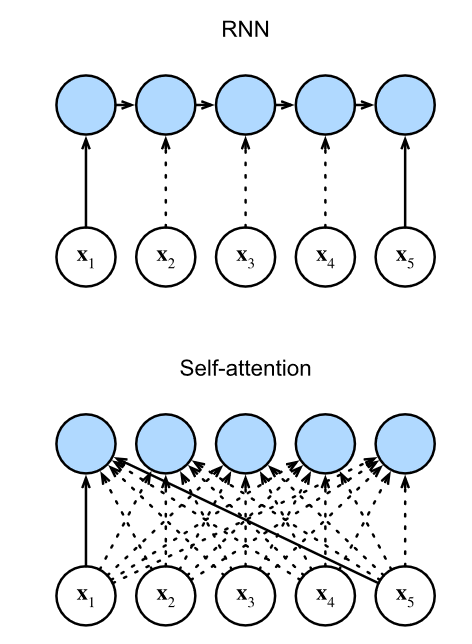
\includegraphics[width=0.5\textwidth]{assets/pics/rnn-compare-selfattention.png}
		\captionsource{Perbandingan RNN dan \f{self-attention} dalam menghasilkan representasi vektor kontekstual. Pada RNN, representasi vektor kontekstual setiap token bergantung pada perhitungan token sebelumnya. Pada \f{self-attention}, representasi vektor kontekstual setiap token dihitung secara independen dan paralel.}{\citep{zhang2023dive}.}
		\label{fig:self-attention-rnn}
	\end{figure}

	\f{Self-Attention layer} adalah \f{layer} yang digunakan \f{transformer} untuk menghasilkan representasi vektor yang kontekstual dari barisan token \f{input}. Berbeda dengan RNN dalam menghasilkan representasi vektor kontekstual, \f{self-attention} tidak memerlukan ketergantungan sekuensial, yang berarti representasi vektor kontekstual setiap tokennya dapat dihitung secara independen dan paralel. \pic~\ref{fig:self-attention-rnn} mengambarkan perbedaan kedua arsitektur dalam menghasilkan representasi vektor kontekstual. Kemampuan Paralelisme dari \f{self-attention} membuat proses komputasi menjadi lebih cepat pada \f{hardware} yang mendukung paralelisme. 

	Perhitungan \f{self-attention} pada \f{transformer} yang digunakan adalah \f{scaled dot product attention} yang telah dijelaskan pada \sect~\ref{sec:scaled-dot-product-attention}. Pada \f{self-attention}, kumpulan vektor kueri $\mathbf{Q}$, vektor kunci $\mathbf{K}$, dan vektor nilai $\mathbf{V}$ adalah vektor yang sama, yaitu \f{embedding} dari token $\mathbf{E}$ yang dijelaskan pada \sect~\ref{sec:token-embedding}. Selain itu, Dimensi dari \f{learned embedding space} $d_{\text{attn}}$ yang digunakan untuk perhitungan nilai atensi adalah $d_{\text{token}}$ yaitu dimensi dari \f{token embedding}. \equ~\ref{equ:self-attention-start} menunjukkan bagaimana \f{self-attention} dihitung.
	\begin{align}
		\label{equ:self-attention-start}
		\nonumber
		\text{Self-Attention}(\mathbf{E}) &= \text{Attention}(\mathbf{EW}^q, \mathbf{EW}^k, \mathbf{EW}^v) \\
		&= \text{Softmax}(\frac{\mathbf{E} \mathbf{W}^q (\mathbf{E} \mathbf{W}^k)^{\top}}{\sqrt{d_{attn}}}) (\mathbf{E} \mathbf{W}^v) \in \mathbb{R}^{L \times d_{\text{token}}},
	\end{align}
	dengan $\mathbf{W}^q, \mathbf{W}^k, \in \mathbb{R}^{d_{\text{token}} \times d_{\text{token}}}, \mathbf{W}^v \in \mathbb{R}^{d_{\text{token}} \times d_{\text{token}}}$ adalah matriks bobot.

	\f{self-attention} dapat dikonsepsikan sebagai proses pembentukan representasi token yang kontekstual. Untuk setiap tokennya, \f{self-attention} menghitung keserupaan antara token $\mathbf{E}\mathbf{W}^q$ dengan seluruh token lainnya $\mathbf{E} \mathbf{W}^k$ dengan \f{scaled dot product attention}. Hasil dari \f{scaled dot product attention} adalah vektor yang menunjukkan bobot atensi dari token tersebut terhadap token lainnya. Bobot atensi tersebut kemudian digunakan untuk menghitung rata-rata terbobot dari seluruh token lainnya ($\mathbf{E} \mathbf{W}^v$). Hasil dari rata-rata terbobot tersebut adalah representasi vektor kontekstual dari token tersebut. \pic~\ref{fig:self-attention-example} adalah contoh dari \f{self-attention} yang menghasilkan representasi vektor kontekstual pada token \f{it}. Pada \pic~\ref{fig:self-attention-example} kiri token \f{it} memiliki bobot atensi yang tinggi terhadap token dan \f{animal} sehingga representasi vektor kontekstual dari token \f{it} akan memiliki nilai yang serupa dengan representasi token \f{animal}. Di lain sisi, token \f{it} pada \pic~\ref{fig:self-attention-example} memiliki bobot atensi yang tinggi terhadap token \f{street}.
	\begin{figure}
		\centering
		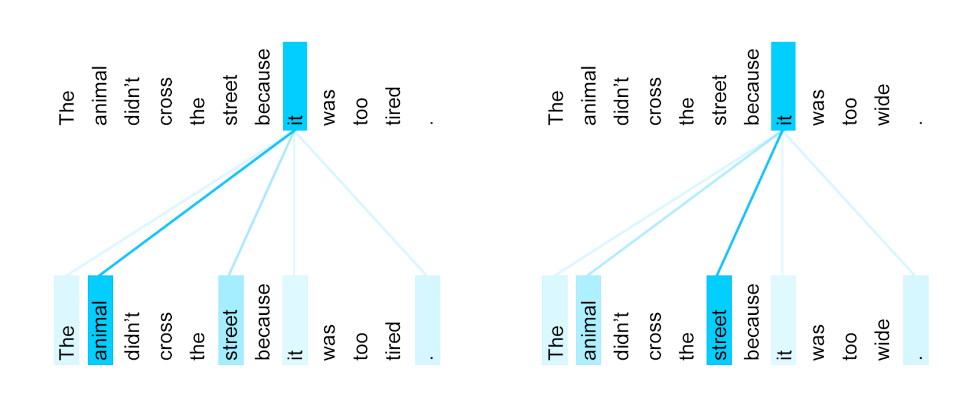
\includegraphics[width=1\textwidth]{assets/pics/self-attn-example.png}
		\captionsource{Ilustrasi \f{self-attention} dalam menghasilkan representasi vektor kontekstual dari barisan token. Representasi vektor dari token \f{it} akan bergantung terhadap barisan token \f{input}.}{\citep{pml1Book}}
		\label{fig:self-attention-example}
	\end{figure}
	
	\subsection{\f{Multi-Head Self-Attention}}
	\begin{figure}
		\centering
		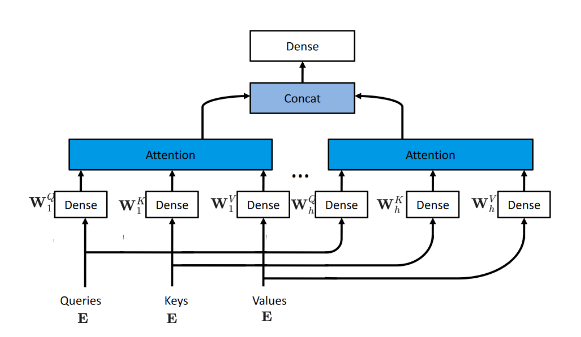
\includegraphics[width=1\textwidth]{assets/pics/MHSA.png}
		\captionsource{Ilustrasi \f{multi-head self-attention} pada \f{transformer}. \f{Multi-head self-attention} menghitung \f{self-attention} sebanyak $h$ kali pada subruang yang berbeda.}{\citep{pml1Book}, telah diolah kembali.}	
		\label{fig:multi-head-self-attention}
	\end{figure}

	\f{Multi-Head Self-Attention} adalah arsiktetur pada \f{transformer} untuk melakukan mekanisme \f{self-attention} beberapa kali pada subruang (\f{learned embedded space}) yang berbeda. dengan melakukan hal tersebut, diharapkan bahwa model dapat menangkap relasi atau keserupaan antar token dari sudut pandang yang berbeda. 

	Secara teknis, \f{embedding} dari barisan token $\mathbf{E}$ akan dipetakan sebanyak $h$ kali dengan \f{linear layer} yang kemudian hasil \f{attention} dari setiap \f{head} akan digabungkan dan dilakukan transformasi sekali lagi dengan \f{linear layer}. \equ~\ref{equ:multi-head-self-attention-start} menunjukkan bagaimana \f{multi-head self-attention} dihitung.
	\begin{align}
		\label{equ:multi-head-self-attention-start}
		\text{MHSA}(\mathbf{E}) &= [\text{head}_1 | \dots | \text{head}_h] \mathbf{W}^O \in \mathbb{R}^{L \times d_{\text{token}}}, \\
		\text{head}_i = \text{Self-Attention}_i(\mathbf{E}) &= \text{Softmax}(\frac{\mathbf{E} \mathbf{W}^q_i (\mathbf{E} \mathbf{W}^k_i)^{\top}}{\sqrt{d_{\text{token}}/h}}) \mathbf{E} \mathbf{W}^v_i  \in  \mathbb{R}^{L \times \frac{d_{\text{token}}}{h}},
	\end{align}
	dengan $\mathbf{W}^q_i, \mathbf{W}^k_i, \mathbf{W}^v_i,\in \mathbb{R}^{\frac{d_{\text{token}}}{h} \times \frac{d_{\text{token}}}{h}}, \mathbf{W}^O \in \mathbb{R}^{d_{\text{token}} \times d_{\text{token}}}$ adalah matriks bobotnya.

	Perhatikan bahwa dimensi dari \f{learned embedding space} menjadi $\frac{d_{\text{token}}}{h}$ untuk setiap \f{head}-nya. Hal ini dilakukan untuk menjaga dimensi dari \f{output} terakhir tetap sama dengan dimensi dari \f{input}, yaitu $d_{\text{token}}$. Selain itu, justifikasi lainnya yang dapat dibuat adalah setiap \f{head} hanya perlu menggunakan dimensi yang lebih kecil dari $d_{\text{token}}$ untuk menangkap ketergantungan antar-token \citep{pi-tau2023transformer}.

	\subsection{\f{Positional Encoding}}
	\label{sec:positional-encoding}
	Mekanisme \f{self-attention} yang dijelaskan sebelumnya tidak memperhatikan informasi mengenai urutan token selama proses komputasinya. Representasi vektor kontekstual dari suatu token akan sama meskipun urutan tokennya berbeda. Lebih tepatnya, mekanisme \f{self-attention} bersifat \f{permutation equivariant}, yaitu untuk \f{token embedding} $\mathbf{E}$ dan matriks permutasi $\mathbf{P}_{\pi}$, \equ~\ref{equ:permutation-equivariant} terpenuhi.
	\begin{align}
	\label{equ:permutation-equivariant}
	\text{Self-Attention}(\mathbf{EP}_{\pi}) &= \text{Self-Attention}(\mathbf{E})\mathbf{P}_{\pi}
	\end{align}
	Namun, urutan dari token penting dalam pemrosesan bahasa alami. Kalimat \code{saya makan nasi} dan \code{nasi makan saya} memiliki makna yang berbeda. Oleh karena itu, informasi mengenai urutan token haruslah diperhatikan dalam pemrosesan bahasa alami.
	
	\cite{transformerori} menambahkan informasi posisi dengan Menjumlahkan \f{token embedding} $\mathbf{E}$ dengan suatu matriks \f{positional encoding} $\mathbf{PE}$. setiap entri dari $\mathbf{PE}$ adalah fungsi sinusoidal dari posisi token  dan dimensi dari \f{token embedding} seperti yang ditunjukkan pada \equ~\ref{equ:positional-encoding-start}.
	\begin{align}
		\label{equ:positional-encoding-start}
		\text{PE}_{ \text {pos }, i}= \begin{cases}\sin \left(\frac{p o s}{10000^{i / d_{\text {token}}}}\right) & \text {jika } i \bmod 2=0 ,\\ \cos \left(\frac{p o s}{10000^{(i-1) / d_{\text {token}}}}\right) & \text { lainnya. }\end{cases}
	\end{align}

	berbeda dengan \cite{transformerori}, \cite{bertori} menggunakan matriks parameter $\mathbf{W}^{pe} \in \mathbb{R}^{L_{\max} \times d_{\text{token}}}$ untuk menghitung matriks \f{positional encoding} $\mathbf{PE} \in \mathbb{R}^{L \times d_{\text{token}}}$ seperti yang ditunjukkan pada \equ~\ref{equ:positional-encoding-learnable-start} hingga \equ~\ref{equ:positional-encoding-learnable-end}. Kekurangan dari pendekatan ini adalah model tidak dapat melakukan inferensi pada barisan token yang lebih panjang dari $L_{\max}$. \pic~\ref{fig:positional-encoding} mengilustrasikan \f{positional encoding} pada \f{transformer}.
	\begin{align}
		\label{equ:positional-encoding-learnable-start}
		\mathbf{pe}_{i} &= [0, 0,\dots, \underbrace{1}_{\text{indeks ke-}i},0, \dots, 0] \mathbf{W}^{pe} \in \mathbb{R}^{d_{\text{token}}}, \\
		\label{equ:positional-encoding-learnable-end}
		 \text{pos}(t) &= \mathbf{PE} = \begin{bmatrix}
			\mathbf{pe}_1 \\
			\mathbf{pe}_2 \\
			\vdots \\
			\mathbf{pe}_L
		\end{bmatrix} \in \mathbb{R}^{L \times d_{\text{token}}}.
	\end{align}
	\begin{figure}

		\centering
		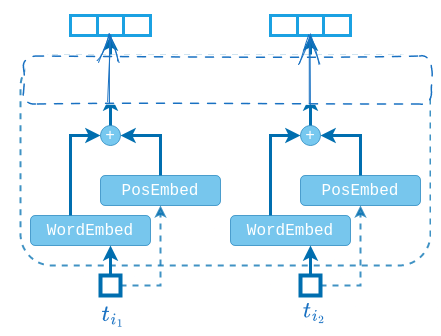
\includegraphics[width=0.5\textwidth]{assets/pics/positional_encoding.png}
		\captionsource{Ilustrasi dari \f{positional encoding} pada \f{transformer}. \f{Positional encoding} ditambahkan pada \f{token embedding} sebelum dijadikan \f{input} untuk \f{transformer}.}{\citep{pi-tau2023transformer}, telah diolah kembali.}
		\label{fig:positional-encoding}
	\end{figure}

\subsection{\f{Position-wise Feed-Forward Network}}
	\begin{figure}
		\centering
		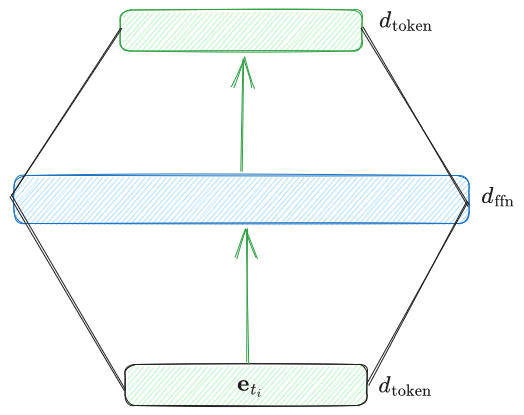
\includegraphics[width=0.5\textwidth]{assets/pics/ffn_transformer.png}
		\caption{Ilustrasi \f{position-wise feed-forward network} pada \f{transformer}.}
		\label{fig:position-wise-feed-forward-network}
	\end{figure}
	\f{Position-wise Feed-Foward Network} adalah \f{feed foward network} dengan dua kali transformasi linear dan sebuah fungsi aktivasi ReLU di antaranya. \pic~\ref{fig:position-wise-feed-forward-network} menunjukkan ilustrasi dari \f{position-wise feed-forward network} dan \equ~\ref{equ:position-wise-feed-forward-network-start} menunjukkan Transformasi yang dilakukan oleh \f{position-wise feed-forward network}.
	\begin{align}
		\label{equ:position-wise-feed-forward-network-start}
		\text{FFN}(\mathbf{X}) &= \max(0, \mathbf{X}\mathbf{W}_1 + \mathbf{b}_1)\mathbf{W}_2 + \mathbf{b}_2 \in \mathbb{R}^{L \times d_{\text{token}}},
	\end{align}
	dengan $\mathbf{W}_1 \in \mathbb{R}^{d_{\text{token}} \times d_{\text{ffn}}}, \mathbf{W}_2 \in \mathbb{R}^{d_{\text{ffn}} \times d_{\text{token}}}, \mathbf{b}_1 \in \mathbb{R}^{d_{\text{ffn}}}, \mathbf{b}_2 \in \mathbb{R}^{d_{\text{token}}}$ adalah matriks bobot dan bias. $d_{\text{ffn}}$ adalah dimensi dari \f{feed forward network} yang digunakan.

	\subsection{Koneksi Residu dan \f{Layer Normalization}}
	\label{sec:layer-normalization}

	Pembaruan parameter model dilakukan pada semua \f{layer} secara serentak setiap iterasi \f{gradient descent}. Ketika parameter suatu \f{layer} mengalami pembaruan, distribusi dari \f{output} yang dihasilkan \f{layer} tersebut juga akan berubah pada iterasi selanjutnya. \f{Layer-layer} selanjutnya harus beradaptasi karena distribusi \f{input} dari \f{layer} tersebut berubah. Fenomena ini disebut \f{internal covariate shift} yang mengakibatkan proses pencarian parameter menjadi lebih lambat.
	
	\f{Layer Normalization} berfungsi untuk mencegah masalah \f{internal covariate shift} di atas dengan membatasi distribusi nilai \f{output} -- yang nantinya menjadi \f{input} pada \f{layer} selanjutnya -- sehingga memiliki variansi 1 dan mean 0. Justifikasi lainnya di balik penggunaan \f{layer normalization} adalah variansi dari \f{input} untuk \f{self-attention layer} haruslah 1 (lihat \sect~\ref{sec:scaled-dot-product-attention}), sehingga variansi dari bobot atensi $\text{Softmax}(\frac{\mathbf{EW}^q (\mathbf{EW}^k)^{\top}}{\sqrt{d_{\text{token}}}})$ akan 1 juga. \equ~\ref{equ:layer-normalization-start} menunjukkan proses kerja dari \f{layer normalization}.
	\begin{align}
		\label{equ:layer-normalization-start}
		\nonumber \text{LayerNorm}(\mathbf{X}) &= (\mathbf{X}-\bm{\mu})\odot \frac{1}{\bm{\sigma}}\\
		&= \begin{bmatrix}
			\frac{x_{11}-\mu_1}{\sigma_1} & \frac{x_{12}-\mu_1}{\sigma_1} & \dots & \frac{x_{1,d_{\text{token}}}-\mu_1}{\sigma_1} \\
			\frac{x_{21}-\mu_2}{\sigma_2} & \frac{x_{22}-\mu_2}{\sigma_2} & \dots & \frac{x_{2,d_{\text{token}}}-\mu_2}{\sigma_2} \\
			\vdots & \vdots & \ddots & \vdots \\
			\frac{x_{L1}-\mu_L}{\sigma_L} & \frac{x_{L2}-\mu_L}{\sigma_L} & \dots & \frac{x_{L,d_{\text{token}}}-\mu_L}{\sigma_L} \\
		\end{bmatrix} \in \mathbb{R}^{L \times d_{\text{token}}}, 
	\end{align}
	dengan keterangan berikut:
	\begin{flalign*}
		\mathbf{X} &= \begin{bmatrix}
			x_{11} & x_{12} & \dots & x_{1,d_{\text{token}}} \\
		x_{21} & x_{22} & \dots & x_{2,d_{\text{token}}} \\
		\vdots & \vdots & \ddots & \vdots \\
		x_{L1} & x_{L2} & \dots & x_{L,d_{\text{token}}} \\
		\end{bmatrix} \in \mathbb{R}^{L \times d_{\text{token}}},&& \\
		\bm{\mu} &= \begin{bmatrix}
		\mu_1 &\dots & \mu_1 \\
		\vdots & \ddots &\vdots \\
		\mu_L & \dots & \mu_L
		\end{bmatrix} \in \mathbb{R}^{L\times d_{\text{token}}},&& \\
		\frac{1}{\bm{\sigma}} &= \begin{bmatrix}
		\frac{1}{\sigma_1} &\dots & \frac{1}{\sigma_1} \\
		\vdots & \ddots &\vdots \\
		\frac{1}{\sigma_L} &\dots & \frac{1}{\sigma_L} \\
		\end{bmatrix} \in \mathbb{R}^{L\times d_{\text{token}}},&& \\
		\mu_i &= \frac{1}{d_\text{token}}\sum_{j=1}^{d_{\text{token}}} x_{ij},\quad i=1,\dots,L,&& \\
		\sigma_i &= \sqrt{\frac{1}{d_{\text{token}}} \sum_{j=1}^{d_{\text{token}}} (x_{ij}-\mu_i)^2}\quad i = 1,\dots, L, && \\
		\odot &= \text{\f{element-wise product.}} &&
	\end{flalign*}

	\begin{figure}
		\centering
		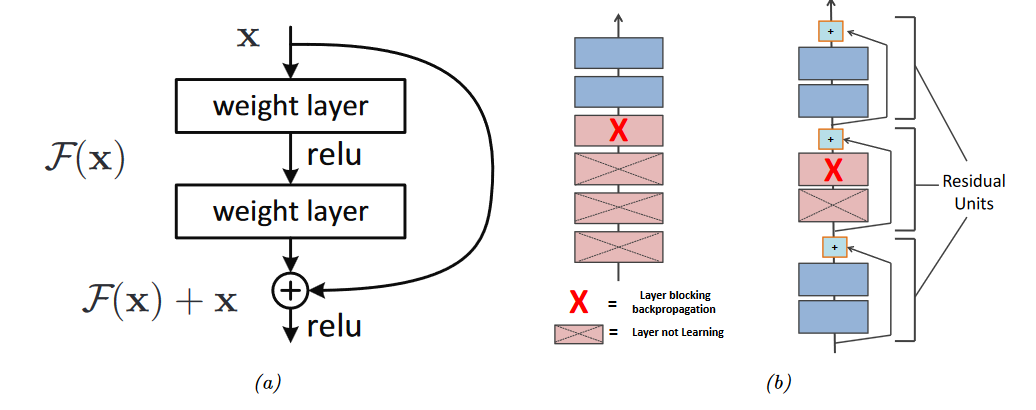
\includegraphics[width=1\textwidth]{assets/pics/residual-connection.png}
		\captionsource{Ilustrasi koneksi residu.}{\citep{pml1Book}}
		\label{fig:residual-connection}
	\end{figure}
	Koneksi Residu adalah koneksi yang menghubungkan \f{output} dari suatu \f{layer} dengan \f{input} dari \f{layer} selanjutnya. Koneksi residu digunakan untuk mengatasi masalah \f{vanishing gradient} yang terjadi pada \f{deep neural network} dengan memperbaiki \f{flow gradient} dari model. Persamaan matematis dari koneksi residu dijelaskan seperti pada \equ~\ref{equ:residual-connection-start}.
	\begin{align}
		\label{equ:residual-connection-start}
		f_l'(\mathbf{x}) &= f_l(\mathbf{x}) + \mathbf{x},
	\end{align}
dengan $f_l(\mathbf{x})$ adalah suatu \f{layer} atau kumpulan \f{layer} pada \f{deep neural network}.
Pada \f{transformer}, \f{residual connection} digunakan sebelum \f{layer normalization}.

	\subsection{Transformer Encoder}
	\label{sec:encoder}

	Dengan menggunakan \f{multi-head self-attention layer}, \f{position-wise feed-forward network layer}, dan \f{layer normalization} dan \f{residual connection} yang sudah dijelaskan sebelumnya, blok \f{encoder} pada \f{transformer encoder} dapat ditulis seperti pada \equ~\ref{equ:transformer-encoder-start} hingga \equ~\ref{equ:transformer-encoder-end}.
	\begin{align}
	\text{EncoderBlock}(\mathbf{X}) &= \mathbf{Z}_2 \in \mathbb{R}^{L \times d_{\text{token}}}, \\
	\mathbf{Z}_2 &= \text{LayerNorm}(\overbrace{\text{FFN}(\mathbf{Z}_1)+\mathbf{Z}_1}^{\text{Koneksi Residu}}), \\
	\mathbf{Z}_1 &= \text{LayerNorm}(\overbrace{\text{MHSA}_h(\mathbf{X}), + \mathbf{X}}^{\text{Koneksi Residu}}),
	\end{align}
	dengan $\mathbf{X} \in \mathbb{R}^{L \times d_{\text{token}}}$ adalah \f{input} dari blok \f{transformer}.

	Terakhir, \f{transformer encoder} adalah komposisi dari beberapa blok \f{encoder}. Untuk \f{input} token $t=(t_1, t_2, \dots, t_L)$, \f{transformer encoder} menghasilkan representasi vektor kontekstual dari setiap tokennya ditunjukkan pada \equ~\ref{equ:transformer-encoder-start} hingga \equ~\ref{equ:transformer-encoder-end}.
	\begin{align}
		\label{equ:transformer-encoder-start} 
		\mathbf{E} &= \text{embed}(t)+ \text{pos}(t) \in \mathbb{R}^{L \times d_{\text{token}}}, \\
		\label{equ:transformer-encoder-end}
		\text{Encoder}(\mathbf{E}) &= \text{EncoderBlock}_n(\text{EncoderBlock}_{n-1}(\dots(\text{EncoderBlock}_1(\mathbf{E})))) \in \mathbb{R}^{L \times d_{\text{token}}}.
	\end{align}
	\begin{figure}
		\centering
		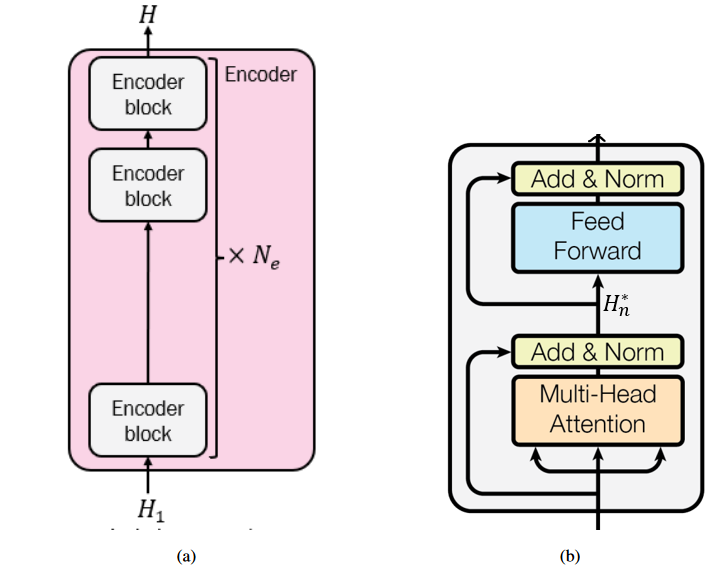
\includegraphics[width=0.5\textwidth]{assets/pics/final-transformers-encoder.png}
		\caption{Ilustrasi \f{transformer encoder}. (a) \f{Transformer encoder}, (b) \f{encoder} blok.}
		\label{fig:transformer-encoder}
	\end{figure}

\section{\f{Bidirectional Encoder Representations from Transformers} (BERT)}
\f{Bidirectional Encoder Representations from Transformers} (BERT) adalah \f{transformers encoder} yang telah dilatih sebelumnya (\f{pre-trained}) pada tugas \f{Masked Language Model} dan \f{Next Sentence Prediction} \citep{bertori}. \f{Pre-training} BERT dilakukan dengan menggunakan korpus teks yang besar dan dilakukan secara \f{self-supervised} untuk mempelajari informasi umum tentang statistik bahasa dan mempelajari representasi vektor kata yang kontekstual. Pengunaan BERT mengikuti prinsip \f{transfer learning}, yaitu model yang sudah dilatih sebelumnya pada tugas tertentu -- dengan jumlah data yang besar -- dapat digunakan untuk tugas lainnya dengan hanya menggunakan sedikit data latih. Model $\text{BERT}_{\text{BASE}}$ tersusun atas 12 blok \f{encoder} dengan dimensi \f{token embedding} $d_{\text{token}}$ sebesar 768, 12 \f{attention heads} pada setiap blok \f{encoder}-nya, 110 juta parameter dan panjang barisan token maksimal $L_{\max}$ sebesar 512.

\subsection{Representasi Input}

Model BERT menghasilkan representasi vektor kontekstual dari token dengan \f{transformer encoder}. \f{Input} dari \f{transformer encoder} berupa vektor numerik sehingga teks harus diubah mengikuti format tersebut. \f{Input} dari model BERT adalah penjumlahan dari \f{token embedding} (lihat \sect~\ref{sec:token-embedding}), \f{segment embedding}, dan \f{position embedding} (lihat \sect~\ref{sec:positional-encoding}).

\f{Token embedding} didapatkan dengan terlebih dahulu memecah teks menjadi kumpulan token. Proses pemecahan teks ini dinamakan proses \f{tokenizing}. \f{Tokenizing} pada BERT dilakukan dengan algoritma \f{WordPiece} yang dikembangkan oleh \cite{tokenizer}.

Dalam proses \f{tokenizing}, teks dipecah menjadi kata atau subkata -- kata-kata yang tidak terdaftar pada kosakata yang dipecah menjadi subkata. Sebagai contoh, misalkan kata \code{etiopia} tidak terdaftar pada kosakata, kata tersebut akan dipecah menjadi subkata \code{eti} dan \code{\#\#opia}, dengan subkata \code{eti} dan \code{pia} terdaftar pada kosakata. Simbol \code{\#\#} menandakan bahwa subkata tersebut merupakan subkata dari kata sebelumnya. Untuk suatu \f{input} berupa teks seperti \code{apa nama ibukota etiopia}, proses \f{tokenizing} mengubah teks tersebut menjadi barisan token (\code{apa}, \code{nama}, \code{ibu}, \code{kota}, \code{eti}, \code{\#\#opia}). 

Setelah proses \f{tokenizing}, token khusus \code{[CLS]} dan \code{[SEP]} ditambahkan di awal dan akhir barisan token sehingga barisan token menjadi (\code{[CLS]}, \code{apa}, \code{nama}, \code{ibu}, \code{kota}, \code{eti}, \code{\#\#opia}, \code{[SEP]}). Token \code{[CLS]} digunakan sebagai representasi dari seluruh kalimat dan token \code{[SEP]} digunakan sebagai pemisah antar kalimat.

Selanjutnya, setiap token pada barisan token dipetakan ke vektor numerik seperti yang dijelaskan pada \sect~\ref{sec:token-embedding}. Hasil \f{token embedding} berupa vektor numerik yang dapat merepresentasikan suatu kata. Untuk menyimpan representasi vektor dari seluruh kosakata, BERT menggunakan matriks \f{token embedding} yang dipelajari ketika proses \f{pre-training} yang berukuran $|\mathcal{T}| \times d_{\text{token}}$ dengan $|\mathcal{T}|$ adalah ukuran kosakata. \tab~\ref{tab:token-embeddings} menunjukkan ilustrasi dari pemetaan \f{token embedding} pada BERT.
\begin{table}
	\centering
	\caption{Ilustrasi pemetaan \f{token embedding} pada BERT.}
	\label{tab:token-embeddings}
	\begin{tabular}{|c|c|c|}
		\hline
		\textbf{Token} & \textbf{Token ID} & \textbf{\f{Token Embedding}} \\
		\hline
		saya & 0 & [-0.0124, -0.0556, -0.0235, \dots, -0.0168, -0.0401, -0.0107] \\
		apa & 1 & [-0.0112, -0.054, -0.0245, \dots, -0.0168, -0.0401, -0.0107] \\
		kamu & 2 & [-0.0124, -0.0556, -0.0235, \dots, -0.0168, -0.0401, -0.0107] \\
		\vdots & \vdots & \vdots \\
		opia & 508 & [-0.0124, -0.0556, -0.0235, \dots, -0.0168, -0.0401, -0.0107] \\
		nasi & 509 & [-0.0218, -0.0556, -0.0135, \dots, -0.0043, -0.0151, -0.0249] \\
		\vdots & \vdots & \vdots \\
		eti & 5000 & [-0.0124, -0.0556, -0.0235, \dots, -0.0168, -0.0401, -0.0107] \\
		\vdots & \vdots & \vdots \\
		\hline
	\end{tabular}
\end{table}

\f{Segment embedding} digunakan sebagai penanda bagian yang berbeda pada suatu barisan token.  Sebagai contoh, pada permasalahan \f{question answering} (\f{QA}), \f{input} pertanyaan direpresentasikan oleh barisan token $A$ dan paragraf konteks direpresentasikan oleh barisan token $B$. Setiap \f{segment} dipisahkan oleh token khusus \code{[SEP]}. Setiap token yang berada pada \f{segment} yang sama akan memiliki vektor numerik yang identik pada \f{segment embedding}. Untuk menyimpan representasi vektor dari setiap \f{segment}, BERT menggunakan matriks \f{segment embedding} yang dipelajari ketika proses \f{pre-training} yang berukuran $2 \times d_{\text{token}}$. \tab~\ref{tab:segment-embeddings} menunjukkan ilustrasi dari pemetaan \f{segment embedding} pada BERT.
\begin{table}
	\centering
	\caption{Ilustrasi pemetaan \f{segment embedding} pada BERT.}
	\label{tab:segment-embeddings}
	\begin{tabular}{|c|c|}
		\hline
		\bo{\f{Segment}} & \bo{\f{Segment Embedding}} \\
		\hline
		0 & [0.0004, 0.011, 0.0037, \dots, -0.0066, -0.0034, -0.0086] \\
		1 & [0.0011, -0.003, -0.0032, \dots, 0.0047, -0.0052, -0.0112] \\
		\hline
	\end{tabular}
\end{table}

\f{Positional embedding} digunakan untuk menghilangkan sifat permutasi \f{equivariant} pada barisan token yang telah dijelaskan pada \sect~\ref{sec:positional-encoding}. Untuk menyimpan representasi vektor dari setiap posisi token, BERT menggunakan matriks \f{positional embedding} yang dipelajari ketika proses \f{pre-training} yang berukuran $L_{\max} \times d_{\text{token}}$, dengan $L_{\max}$ adalah panjang maksimal barisan token. \tab~\ref{tab:positional-embeddings} menunjukkan ilustrasi dari pemetaan \f{positional embedding} pada BERT.
\begin{table}
	\centering
	\caption{Ilustrasi pemetaan \f{positional embedding} pada BERT.}
	\label{tab:positional-embeddings}
	\begin{tabular}{|c|c|}
		\hline
		\bo{Posisi Token} & \bo{\f{Position Embedding}} \\
		\hline
		0 & [0.0175, -0.0256, -0.0366, \dots , 0.0, 0.0007, 0.0154] \\
		1 & [0.0078, 0.0023, -0.0194, \dots, 0.0289, 0.0298, -0.0053] \\
		2 & [-0.0113, -0.002, -0.0116, \dots, 0.0149, 0.0187, -0.0073] \\
		509 & [0.0174, 0.0035, -0.0096, \dots, 0.003, 0.0004, -0.0269] \\
		510 & [0.0217, -0.006, 0.0147, \dots, -0.0056, -0.0126, -0.0281] \\
		511 & [0.0026, -0.0233, 0.0055, \dots, 0.0175, 0.0275, -0.0777] \\
		\hline
	\end{tabular}
\end{table}

\f{Input} dari model BERT adalah hasil penjumlahan dari \f{token embedding}, \f{segment embedding}, dan \f{positional embedding}. Pada penelitian ini, Proses pembentukan \f{input embedding} tersebut diasumsikan menjadi bagian dari fungsi BERT. Oleh karena itu, fungsi $\text{BERT}$ didefinisikan sebagai fungsi yang menerima suatu barisan token (\code{[CLS]}, $t_1, t_2, \dots, t_L$, \code{[SEP]}) dan menghasilkan barisan vektor kontekstual ($\mathbf{T}_{\text{\code{[CLS]}}}, \mathbf{T}_{t_1}, \mathbf{T}_{t_2}, \dots, \mathbf{T}_{t_L}, \mathbf{T}_{\text{\code{[SEP]}}}$) seperti yang ditunjukkan pada \equ~\ref{equ:bert-input-start} dan \pic~\ref{fig:input-representation}.
\begin{align}
	\label{equ:bert-input-start}
	\text{BERT}((\text{\code{[CLS]}}, t_1, t_2, \dots, t_L, \text{\code{[SEP]}})) &= (\mathbf{T}_{\text{\code{[CLS]}}}, \mathbf{T}_{t_1}, \mathbf{T}_{t_2}, \dots, \mathbf{T}_{t_L}, \mathbf{T}_{\text{\code{[SEP]}}}).
\end{align}
\begin{figure}
	\centering
	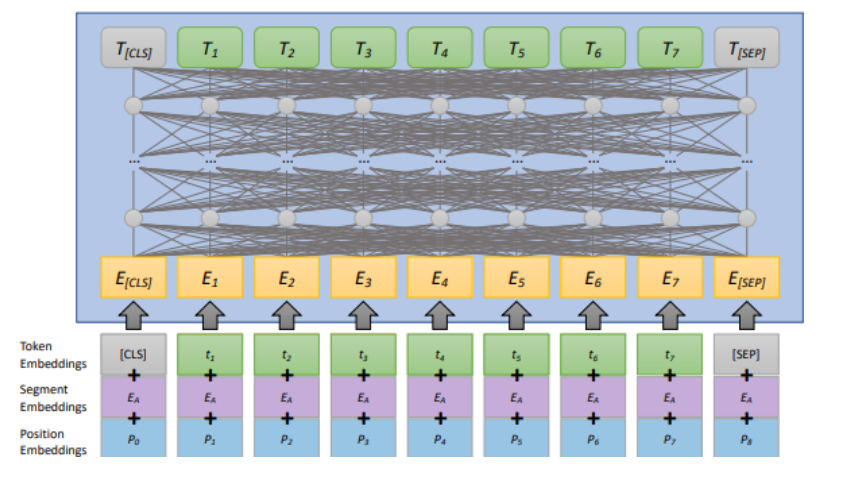
\includegraphics[width=0.75\textwidth]{assets/pics/representasibert.png}
	\captionsource{Ilustrasi dari representasi \f{input} pada BERT. Barisan kata diubah menjadi \f{token}, \f{segment}, dan \f{positional embedding}. Jumlahan \f{embedding} ini menghasilkan \f{embedding} \f{input}, yang melewati 12 blok \f{transformer encoder}. Representasi kontekstual vektor kata diambil dari blok terakhir.}{\citep{textrankingsurvey}.}
	\label{fig:input-representation}
\end{figure}

\subsection{\f{pre-traning} BERT}

	Pada tahap \f{pre-traning}, BERT dilatih pada dua tugas \f{self-supervised} dengan jumlah data yang besar, yaitu \f{Masked Language Model} dan \f{Next Sentence Prediction} yang masing-masing akan dijelaskan pada \sect~\ref{sec:masked-language-model} dan \sect~\ref{sec:next-sentence-prediction}. proses \f{pre-training} menggunakan paragraf-paragraf pada korpus teks yang besar, yaitu Wikipedia dengan 2.5 Miliar kata dan BookCorpus dengan 800 juta kata.


	\subsubsection{\f{Masked Language Model} (MLM)}
	\label{sec:masked-language-model}

	\begin{figure}
		\centering
		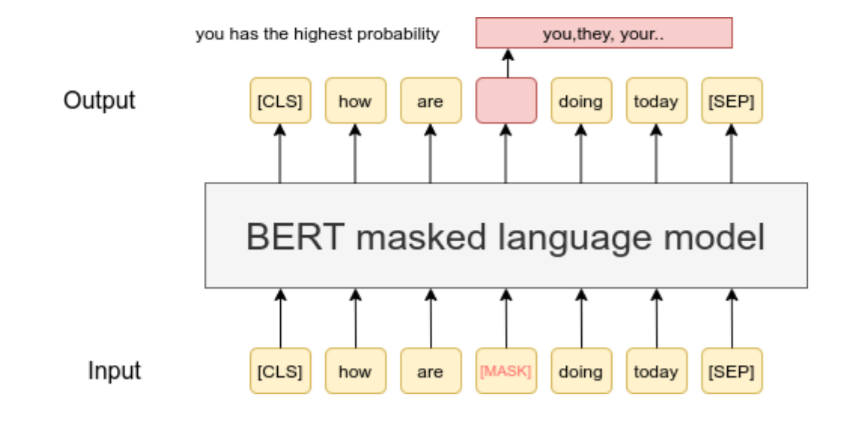
\includegraphics[width=1\textwidth]{assets/pics/MLM.png}
		\caption{Ilustrasi \f{Masked Language Modeling} (MLM) pada BERT. sebuah kata (token) secara acak di-hilangkan (\f{mask}) dan model diminta untuk menebak kata yang dihilangkan tersebut.}
		\label{fig:masked-language-model}
	\end{figure}

	Tugas \f{Masked Language Model} (MLM) adalah tugas untuk memprediksi token yang dihilangkan (\f{masking}) pada suatu kalimat. Sebagai contoh, pada kalimat \code{Let's make [MASK] chicken! [SEP] It [MASK] great with orange sauce}, model harus memprediksi token \code{fried} dan \code{tastes} pada token yang dihilangkan (\code{[MASK]}) tersebut.


	memprediksi kata yang dihilangkan memaksa \f{transformer} untuk memahami sintaks dan konteks dari kalimat tersebut. Sebagai contoh, model harus memahami bahwa kata sifat \code{red} sering terletak sebelum kata benda seperti \code{house} atau \code{car}, tetapi tidak sebelum kata kerja seperti \code{shout}. Selain itu, tugas ini membuat model untuk memperoleh pemahaman umum tentang bahasa alami. Misalnya, setelah dilatih, model akan memberikan probabilitas yang lebih tinggi untuk kata \code{train} yang hilang dalam kalimat \code{[MASK] pulled into the station} daripada kata \code{chicken}.

	Selama proses pelatiahan MLM, sebanyak 15\% dari semua token dipilih untuk dilakukan \f{masking}. 80\% dari token yang terpilih akan diubah menjadi token \code{[MASK]}, 10\% menjadi token acak, dan 10\% lainnya adalah token yang sama.

	\subsubsection{\f{Next Sentence Prediction}}
	\label{sec:next-sentence-prediction}

	Pada tugas \f{Next Sentence Prediction}, model BERT dapat dilatih untuk memprediksi apakah kalimat kedua dari pasangan kalimat adalah kalimat berikutnya. dengan kata lain, untuk pasangan kalimat $(q, d)$, model BERT harus memprediksi apakah kalimat $d$ adalah kalimat berikutnya dari kalimat $q$. \f{Input} dari tugas ini adalah (\code{[CLS] $t_{q_1}, t_{q_2}, \dots, t_{q_n}$ [SEP] $t_{d_1}, t_{d_2}, \dots, t_{d_m}$ [SEP]}) dengan $t_{q_i}$ adalah token dari kalimat $q$ dan $t_{d_i}$ adalah token dari kalimat $d$. \f{Output} dari tugas ini adalah variabel biner yang menunjukkan apakah kalimat $d$ adalah kalimat berikutnya dari kalimat $q$.
	
	Selama proses pelatihan, setengah dari \f{input} tersebut adalah pasangan kalimat di mana kalimat kedua adalah kalimat berikutnya, dan setengah lainnya adalah kalimat yang diambil secara acak dari korpus sebagai kalimat kedua. \pic~\ref{fig:next-sentence-prediction} mengilustrasikan contoh dari tugas \f{next sentence prediction}.

	\begin{figure}
		\centering
		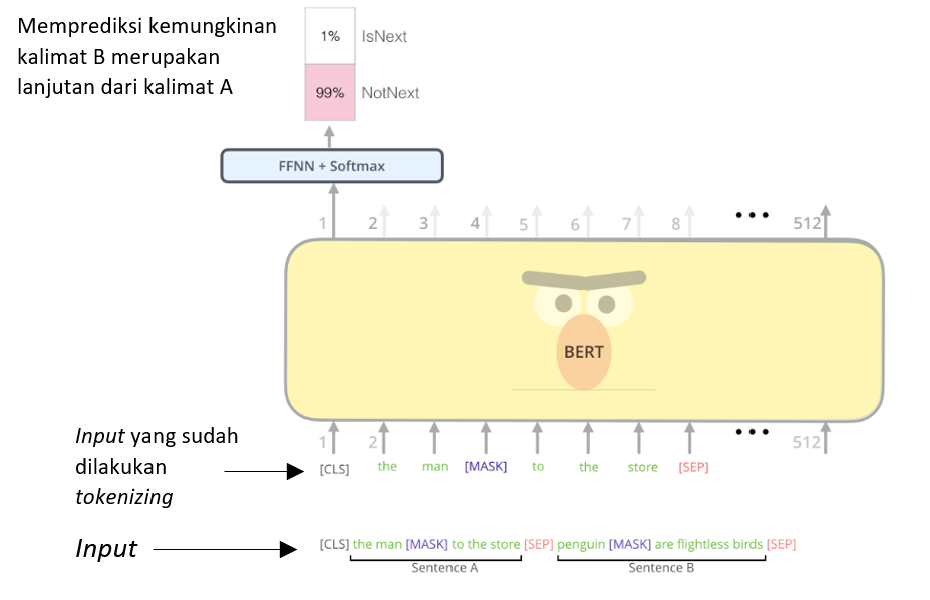
\includegraphics[width=1\textwidth]{assets/pics/Paste.png}
		\caption{Ilustrasi \f{next sentence prediction} pada BERT. Model diminta untuk memprediksi apakah kalimat kedua adalah kalimat berikutnya dari kalimat pertama.}
		\label{fig:next-sentence-prediction}
	\end{figure}

	
	\subsection{BERT untuk Bahasa Indonesia (IndoBERT)}

	Pada penelitian ini, BERT yang digunakan adalah BERT untuk bahasa Indonesia yang sudah dilakukan \f{pre-training} sebelumnya oleh \cite{indobert}. \f{Pre-training} BERT untuk bahasa Indonesia dilakukan dengan menggunakan korpus Wikipedia bahasa Indonesia dengan 74 Juta kata, artikel berita dari Kompas, Tempo, dan Liputan6 dengan 55 Juta kata, dan korpus web bahasa Indonesia dengan 90 Juta kata. Model IndoBERT dilatih selama 2.4 Juta iterasi (180 epoch). Informasi lebih lanjut mengenai model IndoBERT dapat dilihat pada laman \url{https://huggingface.co/indolem/indobert-base-uncased}.


	\subsection{Penggunaan BERT untuk Pemeringkatan Teks}
	Bagian berikut akan mejelaskan penggunaan BERT untuk pemeringkatan teks. Terdapat dua arsitektur yang digunakan, yaitu $\text{BERT}_{\text{CAT}}$ dan $\text{BERT}_{\text{DOT}}$ yang masing-masing akan dijelaskan pada \sect~\ref{sec:bert-cat} dan \sect~\ref{sec:bert-dot}.

	\subsubsection{$\text{BERT}_{\text{CAT}}$}
		\label{sec:bert-cat}

		\begin{figure}
			\centering
			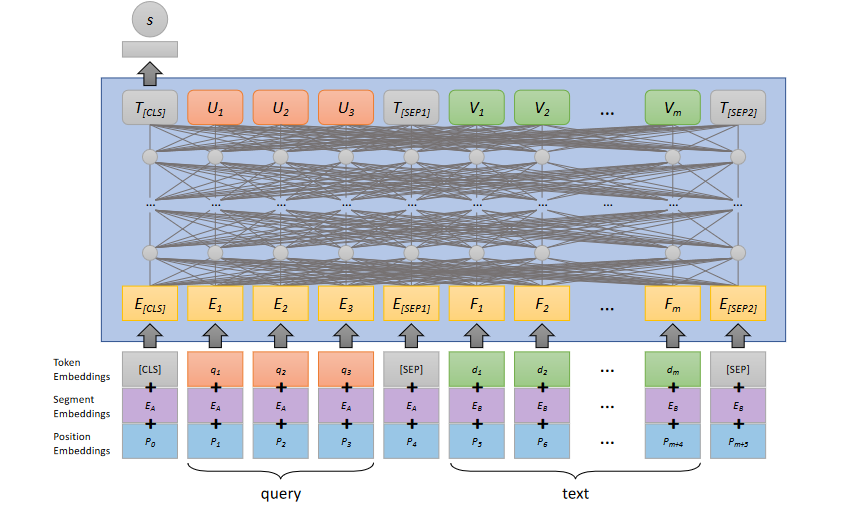
\includegraphics[width=1\textwidth]{assets/pics/bertcat.png}
			\captionsource{$\text{BERT}_{\text{CAT}}$ mengambil kueri dan kandidat teks yang akan diberi skor sebagai \f{input} dan menggunakan BERT untuk klasifikasi melakukan relevansi. Penjumlahan elemen-wise dari token, \f{segment}, dan \f{positional embeddings} membentuk representasi vektor \f{input}. Setiap token input memiliki vektor kontekstual sebagai \f{output} model BERT. \f{Linear layer} menerima representasi akhir token \code{[CLS]} dan menghasilkan skor relevansi teks terkait dengan kueri.}{\citep{textrankingsurvey}.}
			\label{fig:bert-cat}
		\end{figure}

		Salah satu cara pengunaan BERT untuk pemeringkatan teks adalah dengan menggunakan BERT pada
		model untuk melakukan \f{soft classification} nilai relevansi dari pasangan (kueri, teks). Dengan kata lain, skor relevansi dari pasangan (kueri, teks) adalah probabilitas bahwa teks tersebut relevan dengan kueri seperti yang ditunjukkan pada \equ~\ref{equ:bert-cat-start} hingga \equ~\ref{equ:bert-cat-end}.
		\begin{align}
			\label{equ:bert-cat-start}
			\text{score}(q,d) &= P(\text{relevance} = 1 | q, d) = \sigma\left(  \mathbf{h}_{\text{[CLS]}} \mathbf{W}^{\text{CLS}}+\mathbf{b}^{\text{CLS}} \right) \in (0,1), \\
			\label{equ:bert-cat-end}
			\mathbf{h}_{\text{\code{[CLS]}}} &= \text{BERT}((\text{\code{[CLS]}}, q, \text{\code{[SEP]}}, d, \text{\code{[SEP]}}))_{\text{\code{[CLS]}}} \in \mathbb{R}^{d_{\text{token}}},
		\end{align}
		dengan $\mathbf{W}^{\text{CLS}} \in \mathbb{R}^{d_{\text{token} \times 1}}$ dan $\mathbf{b}^{\text{CLS}} \in \mathbb{R}$ adalah matriks bobot dan bias yang digunakan untuk melakukan \f{classification}, dan $\sigma$ adalah fungsi sigmoid.

		Untuk suatu kueri $q$ dan kumpulan teks $D = \{d_1, d_2, \dots, d_n\}$, perlu dilakukan perhitungan skor relevansi untuk setiap pasangan $(q, d_i)$ dengan $i=1,\dots,n$ sebelum dilakukan pemeringkatan. Hal ini menjadi masalah untuk jumlah dokumen yang besar karena setiap perhitungan skor relevansi dengan $\text{BERT}_{\text{CAT}}$ membutuhkan waktu yang lama. Oleh karena itu, $\text{BERT}_{\text{CAT}}$ biasanya digunakan sebagai \f{reranker} dari sistem pemeringkatan teks. Teks yang akan diberikan skor relevansinya oleh $\text{BERT}_{\text{CAT}}$ adalah teks yang sudah dipilih oleh sistem pemeringkatan teks yang lebih efisien seperti {BM25} -- biasanya $k = 100, 1000$ teks teratas dipilih oleh {BM25}. \pic~\ref{fig:bert-cat-withbm25} mengilustrasikan arsitektur \f{retrieve} dan \f{rerank}.

		\begin{figure}
			\centering
			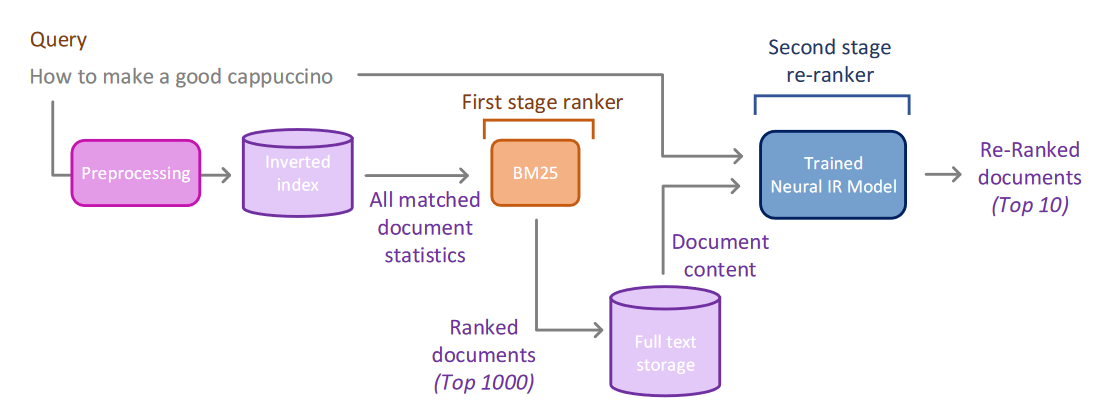
\includegraphics[width=1\textwidth]{assets/pics/neural-ir.png}
			\captionsource{Arsitektur \f{retrieve and rerank}. \f{First-stage retrieval} dilakukan oleh {BM25} dan \f{reranking} dilakukan oleh model \f{scoring} yang lebih kompleks seperti $\text{BERT}_{\text{CAT}}$.}{\citep{irlecture}.}
			\label{fig:bert-cat-withbm25}
		\end{figure}

		\subsubsection{$\text{BERT}_{\text{DOT}}$}
		\label{sec:bert-dot}
		\begin{figure}
			\centering
			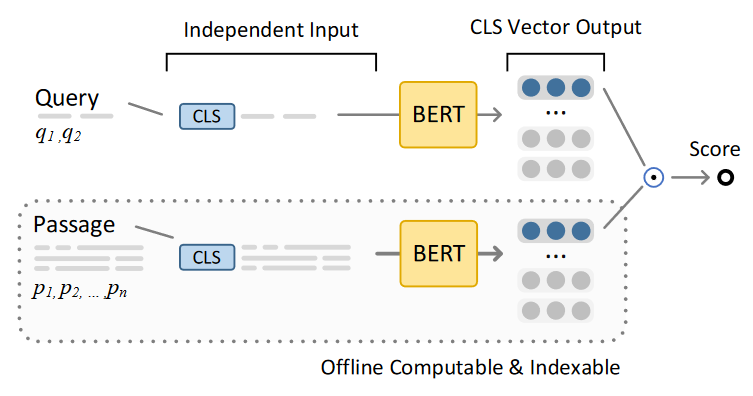
\includegraphics[width=1\textwidth]{assets/pics/bertdot.png}
			\captionsource{$\text{BERT}_{\text{DOT}}$ memetakan kueri dan kandidat teks ke dalam ruang vektor yang sama dan menghitung skor relevansi dengan melakukan \f{dot product} antara vektor representasi kontekstual dari kueri dan teks.}{\citep{irlecture}.}
			\label{fig:bert-dot}
		\end{figure}

		Berbeda dengan $\text{BERT}_{\text{CAT}}$, $\text{BERT}_{\text{DOT}}$ tidak melakukan \f{soft classification} untuk setiap pasangan (kueri, teks). $\text{BERT}_{\text{DOT}}$ menghitung skor relevansi dari pasangan (kueri, teks) dengan melakukan \f{dot product} antara vektor representasi kontekstual dari kueri dan teks seperti yang ditunjukkan pada \equ~\ref{equ:bert-dot-start} hingga \equ~\ref{equ:bert-dot-end}.
		\begin{align}
			\label{equ:bert-dot-start}
			\text{score}(q,d) &= \mathbf{q}_{\text{\code{[CLS]}}} \cdot \mathbf{d}_{\text{\code{[CLS]}}} \in \mathbb{R}, \\
			\mathbf{q}_{\text{\code{[CLS]}}} &= \text{BERT}((\text{\code{[CLS]}}, q, \text{\code{[SEP]}}))_{\text{\code{[CLS]}}} \in \mathbb{R}^{d_{\text{token}}}, \\
			\mathbf{d}_{\text{\code{[CLS]}}} &= \text{BERT}((\text{\code{[CLS]}}, d, \text{\code{[SEP]}}))_{\text{\code{[CLS]}}} \in \mathbb{R}^{d_{\text{token}}}.
			\label{equ:bert-dot-end}
		\end{align}

		Salah satu kelebihan dari $\text{BERT}_{\text{DOT}}$ adalah vektor representasi $\mathbf{d}_{\text{\code{[CLS]}}}$ dari teks dapat diindeks terlebih dahulu dan disimpan dalam memori. Akibatnya, kita hanya perlu menghitung $\mathbf{q}_{\text{\code{[CLS]}}}$ sekali, dan dapat menghitung skor relevansi untuk setiap pasangan (kueri, teks) dengan melakukan \f{dot product} antara $\mathbf{q}_{\text{\code{[CLS]}}}$ dan $\mathbf{d}_{\text{\code{[CLS]}}}$ yang sudah disimpan dalam memori sebelumnya. \pic~\ref{fig:dense-retrieval} mengilustrasikan arsitektur pemeringkatan dengan $\text{BERT}_{\text{DOT}}$.


		\begin{figure}
			\centering
			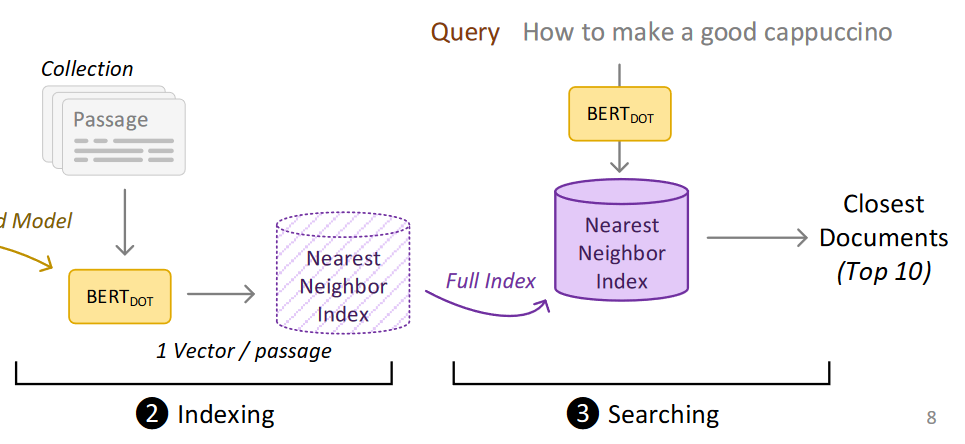
\includegraphics[width=1\textwidth]{assets/pics/dense-retrieval.png}
			\captionsource{Arsitektur pemeringkatan dengan $\text{BERT}_{\text{DOT}}$. Vektor representasi dari setiap teks dapat diindeks terlebih dahulu dan disimpan dalam memori dan skor relevansi dapat dihitung dengan melakukan \f{dot product} antara vektor representasi kueri dan teks.}{\citep{irlecture}.}
			\label{fig:dense-retrieval}
		\end{figure}